%%%%%%
% HRI 2022 Final Project Report 
%%%%%%%

%%%%%%%%%%%%%%%%%%%%
% Abstract
%%%%%%%%%%%%%%%%%%%%
\begin{abstract}

Provide a brief summary of: 
What problem do you aim to address?
Why is this problem an important application? 
What is your proposed approach? 
How does the proposed approach compare to prior work? 
Describe what dataset used to train and evaluate the proposed machine learning models used and provide sources. 
Describe the design of the front- and back-end of the application. 
How will you evaluate the proposed machine learning models including metrics? 
What are the expected findings?
What impacts does this project have on the machine learning field broadly?




\end{abstract}

\begin{IEEEkeywords}
component, formatting, style, styling, insert
\end{IEEEkeywords}

%%%%%
% Section 1: Introduction
%%%%%
\section{Introduction}

Motivation: What problem are you tackling? Why is it interesting/important? What application will you develop and why is it useful? 

Technical focus: What type of machine learning methods are used in the proposed approach and why is it well suited to address the problem. What is particularly unique or novel about your approach? 

Prior Work: Discuss prior work relevant to the proposed work. How is prior work different and similar to the proposed work?

Machine Learning Pipeline: Provide a brief overview of your proposed machine learning pipeline including data exploration, preprocessing, model training and evaluation (including expected results) and deployment of the model in an application. 

Impact: Discussion of social impacts and ethical concerns the application might raise.



\begin{figure}[t]
\centerline{
\includegraphics[width=0.4\textwidth]{Figures/robot_figure.png}}
\caption{Add caption here and include reference in the paper.}
\label{fig:label_name1}
\end{figure}

%%%%%
% Section 2: Related Work
%%%%%
\section{Background}

Review prior work relevant to your project and provide a brief background, discuss how your proposed work is similar and different from prior work, and cite sources in bibtex. Google Scholar provides bibtex code. Place the bibtex code in the references.bib file in Overleaf and cite the source (e.g., \cite{example_bibtex_label}). Based on prior work and results, how do you anticipate your proposed approach will compare to prior approaches?

%%%%%
% Section 3: Method
%%%%%
\section{End-to-End ML Pipeline}

\begin{figure}[t]
\centerline{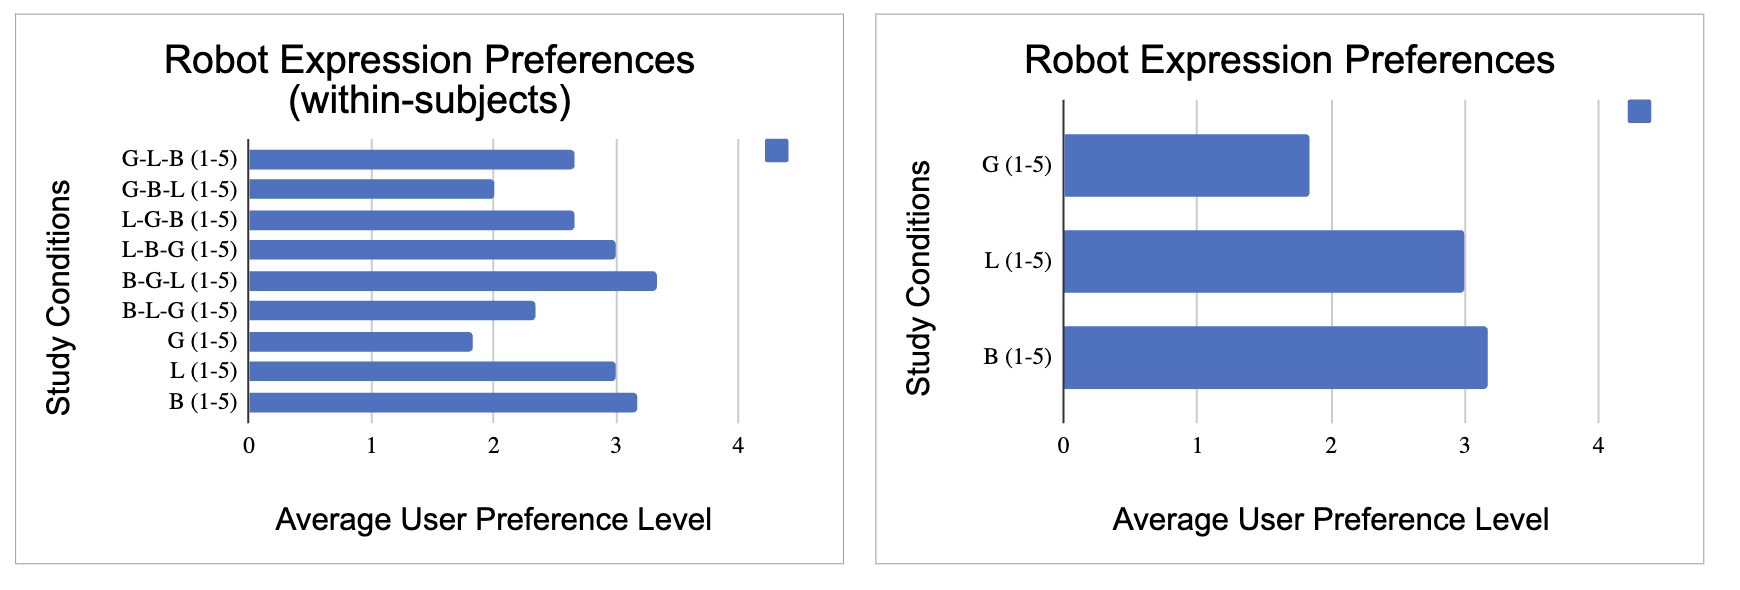
\includegraphics[width=0.5\textwidth]{Figures/study_overview_figure.png}}
\caption{Add caption here and include reference in the paper.}
\label{fig:label_name1}
\end{figure}

\subsection{Back-End}

The Back-End of the web application performs data exploration and preprocessing, model training and evaluation, and launches an application that deploys that trained models. Think of the back-end as the high-level functionality behind website user interface elements (e.g., menus, buttons). For instance, the backend of HW2 trained models when a user pressed a button.

\subsubsection{Data Collection, Exploration & Processing} 

Describe the dataset(s) you plan to use for training machine learning models including the type of data provided, quantity of data, year it was released (if available), source of the dataset (e.g., Kaggle), and how you plan to use it in the project. State whether ground truth labels are provided. If there are none, state how you plan to generate annotations or provide justification for the planned evaluation procedure. At least one dataset is required.

State the preprocessing techniques used to prepare the dataset for ML algorithms. Provide justification for these techniques and how they are used in the next steps of the ML pipeline.


\subsubsection{Methods and Model Training} 

What machine learning techniques are you planning to apply or improve upon and how? Provide justification for why the machine learning approach is well-suited to address the problem. What are the model inputs and outputs? Describe the training and validation procedure including the train/test split. State model parameter settings and justification. Discuss the methods used to avoid model overfitting and underfitting. 

Make sure to describe them in detail and provide enough context for the reader to understand the methods at least at a high level. Provide any background that is necessary for that.


\subsubsection{Model Evaluation} 

escribe the planned experiments, expected outcomes, and error analysis. State the evaluation methods for comparison (at least three required), metrics (at least two required), and hyperparameter settings. The evaluation methods consist of all methods used for comparison. The evaluation metrics assess how well the models perform and can be used to identify over- and underfitting. State whether the metrics used are commonly used for evaluating similar tasks and cite sources. 

Make sure that the setup is described in enough detail for someone else to reproduce your results. Also, if you have an experimental project, make sure to provide a detailed experimental analysis. Things you should consider including: train/test performance, learning curves, model samples, error analyses, ablation analyses, etc. 

Context: Explain how you build upon previous work and how your expected results compare to what has been done previously (be realistic in your prediction).


\subsubsection{Model Deployment} 

Describe the application of proposed project including user inputs and model outputs. Discuss the importance of the application as well as ethical or societal implications of its usage with everyday users.

\subsection{Front-End (Streamlit)}

The Front-End of the web application includes that user interface (UI) layout, user inputs using menus, buttons, and more. Describe the web application layout including the number of pages, outline of page, menus, input widgets, chart elements, etc.

Provide figures to depict the proposed website layout and provide detailed discussion on how the front- and back-end are connected (e.g., training a model by pressing a button). Feel free to be creative and design a clear, concise, and well presented application.


\section{Risk \& Mitigation}

Identify challenges you are anticipating, and how you are planning to mitigate them e.g., programming, model training, and evaluation. 

\section{Expected Outcomes }

State the expected outcomes of the project based on prior work or a high-level inspiration or motivation.

\section{Team Member Contribution}


Each team member is expected to contribute to the final project. Task responsibilities must be clearly stated in terms of front- and back-end development.


\subsection{Technical Components}

Include the team contributions in terms of technical goals of the project such as programming front- and back-end components and algorithms. 

\subsection{Writing Components}

Include the team contributions for writing sections of the final report for all sections. 


